%        File: topology.tex
%     Created: Thu Nov 09 01:00 PM 2006 C
% Last Change: Thu Nov 09 01:00 PM 2006 C
%
% This file is part of Netsukuku
% (c) Copyright 2007 Andrea Lo Pumo aka AlpT <alpt@freaknet.org>
%
% This source code is free software; you can redistribute it and/or
% modify it under the terms of the GNU General Public License as published 
% by the Free Software Foundation; either version 2 of the License,
% or (at your option) any later version.
%
% This source code is distributed in the hope that it will be useful,
% but WITHOUT ANY WARRANTY; without even the implied warranty of
% MERCHANTABILITY or FITNESS FOR A PARTICULAR PURPOSE.
% Please refer to the GNU Public License for more details.
%
% You should have received a copy of the GNU Public License along with
% this source code; if not, write to:
% Free Software Foundation, Inc., 675 Mass Ave, Cambridge, MA 02139, USA.
%

\documentclass[a4paper]{article}
\usepackage{color,graphicx}
\usepackage{amsmath}
\usepackage{amsthm}
\usepackage{amssymb}
\usepackage{amsfonts}
\RequirePackage{ifpdf} % running on pdfTeX?
\ifpdf
\usepackage[pdftex,bookmarks=true,
		   bookmarksnumbered=false,
		   bookmarksopen=false,
		   colorlinks=true,
		   linkcolor=webred] {hyperref}
\definecolor{webgreen}{rgb}{0, 0.5, 0} % less intense green
\definecolor{webblue}{rgb}{0, 0, 0.5} % less intense blue
\definecolor{webred}{rgb}{0.5, 0, 0}   % less intense red
\else
\newcommand{\href}[2]{ #1 }
\fi

%%%% Misc
\newcommand{\T}[1]{\textrm{#1}}
\newcommand{\see}[1]{\T{[\ref{#1},pg.\pageref{#1}]}}
\newcommand{\vedi}[1]{\T{vedi \see{#1}}}
\newcommand{\pgra}[1]{\left\{#1\right\}}
\newcommand{\pqua}[1]{\left[#1\right]}
\newcommand{\pton}[1]{\left(#1\right)}
\newcommand{\pass}[1]{\Big|#1\Big|}
\newcommand{\sist}[1]{{ \begin{cases} #1 \end{cases} }}
\newcommand{\eal}[1]{{\begin{align*} #1 \end{align*}}}
\def\ove#1{{\overline{#1}}}
\newcommand{\qq}{\qquad}
%% Defs
\def\*{{\times}}
\def\|{{\;\lor\;}}
\def\&{{\;\land\;}}
\def\-{{\setminus}}
\def\0{{\emptyset}}
\def\8{{\infty}}
\def\v{{\cup}}
\def\^{{\cap}}
\def\<{{\;\Leftarrow\;}}
\def\>{{\;\Rightarrow\;}}
\def\={{\;\Leftrightarrow\;}}
\def\({{\subseteq}}
\def\){{\supseteq}}
\def\'{{\;\;\;}}
\def\,{{,\;}}




\title{Netsukuku topology}
\author{http://netsukuku.freaknet.org\\AlpT (@freaknet.org)}
\begin{document}
\maketitle
\begin{abstract}
	In this document, we describe the hierarchical structure of the Netsukuku
	topology. Moreover, we show how it is possible to use the QSPN v2 on
	the high levels of the hierarchy.
\end{abstract}
\pagenumbering{roman}
\pagebreak
\begin{small}
  This document is part of Netsukuku.\\
  Copyright \copyright 2007 Andrea Lo Pumo aka AlpT $<$alpt@freaknet.org$>$.
  All rights reserved.

  This document is free; you can redistribute it and/or modify it
  under the terms of the GNU General Public License as published by
  the Free Software Foundation; either version 2 of the License, or
  (at your option) any later version.

  This document is distributed in the hope that it will be useful, but
  WITHOUT ANY WARRANTY; without even the implied warranty of
  MERCHANTABILITY or FITNESS FOR A PARTICULAR PURPOSE\@.  See the GNU
  General Public License for more details.

  You should have received a copy of the GNU General Public License
  along with this document; if not, write to the Free Software
  Foundation, Inc., 675 Mass Ave, Cambridge, MA 02139, USA.
\end{small}

\clearpage
\tableofcontents
\clearpage
\pagenumbering{arabic}


\section{Preface}
\label{sec:preface}

We're assuming that you already know the basics of the QSPN. If not, read the
QSPN document first: \cite{qspndoc}.

\section{The general idea}
\label{sec:general_idea}

The aim of Netsukuku is to build a (physical) scalable mesh network, completely
distributed and decentralised, anonymous and autonomous.

The software, which must be executed by every node of the net, has to be
unobtrusive. It has to use very few CPU and memory resources, in this way it
will be possible to run it inside low-performance computers, like Access Points,
embedded devices and old computers.

If this requirements are met, Netsukuku can be easily used to build a worldwide
distributed, anonymous and not controlled network, separated from the
Internet, without the support of any servers, ISPs or control authorities.

\section{Basic definitions}

\begin{description}
	\item[Node] We call \emph{node} any computer that is hooked up to the
		Netsukuku network.
	\item[Rnode] stands for \emph{in-Range Node}: given a node X, it is any other
		node directly linked to X, i.e. it's a neighbour of X.
	\item[Map] A map is a file, kept by each node, which contains all the
		necessary information about the network, f.e. routes and nodes
		status.
	\item[REM] stands route \emph{Route Efficiency Measure}. It is 
		a value that indicates the quality of a route. 
		REM can be calculated in various ways, f.e. by taking in
		account the total rtt and the bw capacity of the route.  We denote the REM of
a route $r$ as $REM(r)$. If $r$ is a better route than $s$, then
$rem(r)>rem(s)$.

\end{description}
Example:\\
\begin{figure}[h]
	\begin{center}
		\includegraphics[scale=0.5]{fig/segABC}
	\end{center}
	\caption{The nodes A,B and C}
\end{figure}
A is the rnode of B.\\
B is the rnode of A and C.\\
C is the rnode of B.

\section{Network topology}
\label{sec:net_topology}

A simple topology, which doesn't impose any structure on the network, can be
memorised with a simple map. In this map, all the information regarding the
nodes of the network have to be memorised. Surely, this kind of map cannot be
utilised by Netsukuku, because it would require too much memory.
For example, even if we store just one route to reach one node and even if
this route costs one byte, we would need 1Gb of memory for a network composed
by $10^9$ nodes (the current Internet).

For this reason, it's necessary to structure the network in a convenient
topology.

\subsection{Hierarchical topology}
\label{sec:fractal_topology}
\subsubsection{Level 1}
First of all we'll subdivide the network in groups of 256 nodes and we'll use
the following definitions:
\label{gnodedef}
\begin{description}
	\item[Gnode] means group node. A group node $G$ is a set of connected
		nodes. Each node of the network belongs to just one gnode. The
		nodes of $G$ are connected in the following sense:
		\eal{&\forall a,b\in G\;\;\exists \T{ a path $a\rightarrow b$ all contained in $G$}}
		In the netsukuku implementation, a gnode contains a maximum of
		256 nodes.\\
		By writing $|G|$ we indicate the number of nodes contained in
		$G$.
	\item[Bnode] stands for border node. It is a node which belongs to a
		gnode G, but that is also directly linked to at least one node
		of another gnode, i.e. some of its rnodes belongs to different
		gnodes than its.\\
		By writing $b \in G$ we mean that the bnode $b$ belongs to the
		gnode $G$.
\end{description}

Example:\\
\begin{figure}[h]
	\begin{center}
		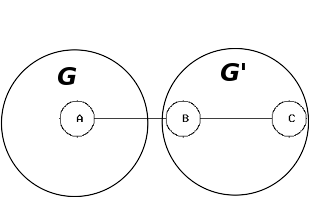
\includegraphics[scale=0.5]{fig/bnode}
	\end{center}
	\caption{The bnode A and B, belonging respectively to the gnode G and
	$G'$}
\end{figure}
$A \in G $, A is a node belonging to the gnode G, its rnode is B.\\
$B \in G'$, B is a node belonging to the gnode $G'$, its rnode is A.\\
A is a bnode of G, while B is a bnode of $G'$.

\subsubsection{Level n}
We further subdivide the network topology in \emph{groups of 256 groups of nodes}
and we continue to name them as gnode.\\
At this point, we repeat recursively this subdivision process until
we can group all the nodes of the network into a single gnode.

Doing so, we've structured the network in $n+1$ levels (from $0$ to $n$).\\
In the base level (level 0), there are 256 single nodes.\\
In the first level (level 1), there are 256 normal gnodes. Each of them
contains 256 single nodes.\\
In the second (level 2), 256 gnodes of level 1 forms a single \emph{group of
groups of nodes}.\\
In the third (level 3), there are 256 groups of 256 groups of 256 groups of
256 nodes.\\
Continuing in this way, we arrive at the last level (level $n$), where there
is a single group which contains the whole network.\\

The QSPN algorithm is able to operate independently on any level,
considering each gnode as a single node of level 0.
For this reason, we can view the Netsukuku topology as a hierarchy, where each
level is composed by single nodes.

\subsubsection*{Example}

Figure \ref{fig:fract_circle}\footnote{this figure has been taken from:
\href{http://www.ian.org/FX/Plugins.html}{http://www.ian.org/FX/Plugins.html}}
is an example of the hierarchical topology of Netsukuku.

\begin{figure}[h]
	\begin{center}
		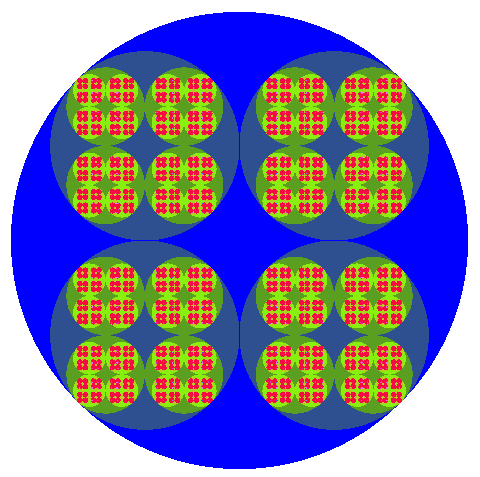
\includegraphics[scale=0.5]{fig/fractal_circle}
	\end{center}
	\caption{An example of the netsukuku topology structure}
	\label{fig:fract_circle}
\end{figure}

In this topology, each gnode contains four nodes, i.e. each group contains
four elements. The network is structured in 6 levels.
\begin{center}
	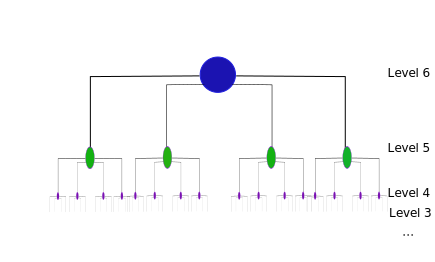
\includegraphics[scale=0.9]{fig/sample-topology-tree}
\end{center}
The red elements, are single nodes (level 0).\\
Four nodes forms a single group of nodes (level 1).\\
A single bright green circle is a 
				  group of groups of nodes (level 2).\\
The dark green circles are        groups of groups of groups of nodes (level 3).\\
The dark blue circle are          groups of groups of groups of groups of
nodes (level 4). \\
Finally, the bright blue circle is the gnode which contains the whole network
(level 5).

\subsubsection{Membership}
Let's assign a numeric ID to each (g)gnode, starting from the last level:
\begin{enumerate}
	\item in the last level ($n$) there's only one giant gnode, thus we assign
		to it the ID ``0''. Our global ID will be:
		\[
		0
		\]
	\item in $n-1$ there are 256 gnodes, which belongs to the gnode 0 of
		level $n$, thus we assign them the IDs from $0$ to $255$.
		The global ID becomes:
		\[
		0\cdot i\quad 0\le  i\le 255
		\]
	\item we repeat the step 2 recursively gaining an ID of this form:
		\[
		0\cdot i_{n-1}\cdot i_{n-2}\cdot \dots \cdot i_0 \quad 0\le i_j\le 255,\;0\le j\le n-1
		\]
	\item since the last level is always $0$, we'll omit it and we'll
		consider only the first $n$ levels.
\end{enumerate}
In a network with a maximum of $2^{32}$ nodes (the maximum allowed by the ipv4),
there would be five levels ($n=4$), where each gnode will be composed by 256 nodes.
Therefore, the ID will be in the usual IP form:
\[
0\dots255\cdot 0\dots255\cdot 0\dots255\cdot 0\dots255
\]
For example, a single node of level 0 of the network is:
\[
3\cdot 41\cdot 5\cdot 12
\]
That said, each gnode of the network belongs to only one combination of gnodes
of the various levels. In our previous example we have:
\begin{align*}
	&g_3=3\\
	&g_2=41\\
	&g_1=5\\
	&g_0=12
\end{align*}
where each $g_i$ corresponds to the gnode ID of the level $i$. Note that $g_0$
is the ID attributed to the single node, at level 0.

Finally, we can assign to each gnode G, of any level, a fingerprint $fg(G)$,
which identifies $G$ in a unique way, indipendently from its ID: two
different, separated gnodes may have the same ID, but not the same
fingerprint. A valid fingerprint is $fg(G)=(uptime(G), rid(G))$, where
$rid(G)$ is a random ID generated at creation time of $G$.

\subsection{Hierarchical map}
The advantages of using a hierarchical topology are clear.\\
The node $N$, instead of memorising information about each node of the whole
network, will keep only that regarding the gnodes where it belongs to.
Suppose the node $N$ had this ID:
\[
g_3\cdot g_2\cdot g_1\cdot g_0
\]
It will store in memory information regarding:
\begin{enumerate}
	\item the 256 single nodes which belongs to its same gnode of level 1,
		or in other words, the 256 nodes of the gnode $g_1$,
	\item the 256 gnodes gnodes which belongs to its same gnode of level
		2, of in other words, the 256 gnodes of the gnode $g_2$,
	\item the 256 gnodes which belongs to the gnode $g_3$.
	\item the 256 gnodes which belongs to the unique gnode $g_4=0$ of the
		last level
\end{enumerate}
Note that doing so, the node $N$ will be blind to all the other gnodes. For
example, it won't know any information regarding the single nodes which belong
to all the other gnodes of level 1 different from $g_1$.\\

Even with this lack of knowledge, as we'll see later, the node $N$ is still
able to reach all the other nodes of the network.
In conclusion, $N$ only needs $256n$ entries in its map, instead of $2^{32}$. 
To clarify the ideas suppose that each entry costs one byte. In the plain
topology we needed $4Gb$, while in the hierarchical one we just need $256\cdot 4\;
b= 1Kb$.

\subsubsection{IP v4 and v6}
Netsukuku is both compatible with ipv4 and ipv6.\\

In ipv4 there are a maximum of $2^{32}$ IPs, thus we have five levels $n=4$.\\
In ipv6 there are a maximum of $2^{128}$ IPs, thus $n=16$.

\subsubsection{Internal and external map}
For simplicity we divide the map of the node $N$, in the \emph{internal map} and in
the \emph{external} one.  The internal map contains information regarding the
nodes belonging to $g_1$. The external map describes all the other levels of
the topology.

\subsection{CIDR routing}
The QSPN, for each level, will build the routes necessary to connect each
(g)node to all the other (g)nodes of the same level. The routes will be saved
in the maps of each node.\\

If the node $N=g_3\cdot g_2\cdot g_1 \cdot g_0$ wants to reach a node $M$ which
belongs to different gnodes, f.e. $M=g_3\cdot g_2\cdot h_1 \cdot h_0$, it will
add a CIDR\cite{CIDR} route in the routing table of the kernel:\\
\emph{all the packets whose destination is $g_3\cdot g_2\cdot h_1 \cdot 0\dots
255$ will be forwarded to the gateway $X$}.\\

We'll see later how the gateway $X$ is chosen.

\section{The internal map and its myopia}
\label{sec:intmyopia}
We define a route $r_N$ of the node $N$ as the following tern:
\eal{&r_N:=(dst, gw, rem)\\
&\T{where }\\
&\qq \T{$dst$ is a node: the destination node of the route}\\
&\qq \T{$gw$ is a node: the gateway of the route}\\
&\qq \T{$rem$ is a number: the REM value of the route}
}
We'll use $ dst(r), gw(r), rem(r)$, to indicate respectively the first, second
and third element of the tern $r$. Let $V_N$ be the set of all neighbours of
$N$.\\
Let $\textbf{R}$ be the set
of all routes of the node $N$ (note \footnote{for simplicity we are considering just one metric for all
the routes. However, it's easy to see that the following
propositions are valid for different metrics (just use a different set
$\textbf{R}_m$ for each metric $m$)}). We can define the following equivalence relation:
\eal{&\forall r,s\in \textbf{R}\;\;\;r\sim s \= dst(r)=dst(s) }
With $\ove r$ we indicate the equivalence class of $r$. Let $B_x(r)$ be the
best route of the routes in $\ove r$ with gateway $x$, where $x\in V_N$, i.e. 
\eal{&
x\in V_N,\;B_x(r)\in \ove r,\;\;rem(B_x(r))= \max \pgra{rem(s)\;|\;s\in\ove
r,\;gw(s)=x}
}
\\
Consider the following subset of $\textbf{R}$:
\eal{&R=\pgra{r \in \textbf{R}\;|\;dst(r) \in G}\\
&\T{where $G$ is the gnode of level 1 such that $N\in G$}
}
At this point we can define the internal map of $N$ as the subset $M\( R$,
where $M=\pgra{B_x(r)\;|\;r\in R,\;x=gw(r)}$. The following property holds:
\eal{& \forall r\in M\;\;\forall s,t\in \ove r\;\T{with}\;s\neq t\;\;\; gw(s)\neq gw(t)
}
Algorithmically,  when the node $N$ wants to save in $M$ a route $s$, which has
the same destination of a route $r\in M$, the following algorithm will be
adopted:
\eal{&\textbf{if}\' \exists t\in \ove r:\;gw(t)=gw(s)\\
&\qq \textbf{if}\' rem(t) < rem(s)\'\T{[s is better than t]}\\
&\qq\qq \T{overwrite t with s;}\\
&\qq \textbf{else}\' \T{do nothing};\\
&\textbf{else}\' \T{save s in $M$;}
}
The reason for the above definitions is that a node $N$, in order 
to reach any other node of the network will just need to know to which of its
neighbours send the packets.\\
A route saved in the internal map it's just a tern, not an ordinate sequence
of nodes, therefore the node $N$ doesn't know its entire path. For this
reason, we can say that the vision of the node $N$ of the entire net is myope,
or local. As we'll see later, this local vision can be easily applied to
higher levels. Note also that the QSPN v2 is indipendent from the above
definitions, i.e. it's way of working doesn't change.


\section{Flat levels}
\label{sec:flat}
From the point of view of the QSPN v2, the levels are ``flattened'', because
the propagation of an ETP \footnote{for more info on the ETP,
see the QSPN document \cite{qspndoc}} inside the whole network is exactly as
before, briefly: a packet is propagated until it is interesting, the
subdvisions of nodes in gnodes are simply ignored . The only
added rule serves to economize space: 

let $T$ be a generic tracer packet and let $\pgra{a_i\;|\;i=1,2,\dots,n}$ be its finite sequence of nodes.
Every subsequence \[\pgra{a_h\in G\;|\;h=i+1,i+2,\dots,j-1}\]
such that $a_i,a_j\notin G$, where $G$ is a gnode of any level, is replaced by
the ID of $G$. The rem associated with the ID of $G$ is the summation of the
rem of every term of the subsequence.\\
This rule is valid for any level, it is called the \emph{group rule}.\\
Some examples:
\begin{enumerate}
	\item The tracer packet
		\eal{&11.22.1,\;11.22.80,\;11.22.35}
		cannot be grouped, because $a_i\in 11.22\;\forall i =1,2,3$
	\item The tracer packet
		\eal{&11.22.1,\;11.22.80,\;11.22.35,\;11.44.13}
		can be grouped in the following tracer packet:
		\eal{&11.22.*,\;11.44.13}
	\item The tracer packet
		\eal{&11.22.1,\;11.22.80,\;11.22.35,\;11.44.13,\;55.32.20}
		can be grouped in the following tracer packet:
		\eal{&11.*,\;55.32.20\'\'(1)}
\end{enumerate}
The description of a route in the external map is local, as in the internal
map (see \ref{sec:intmyopia}). For example, when the node $55.32.12$ receives
the tracer packet $(1)$, it will save the following route:
\eal{&(dst=11.*=\T{any node of the gnode $11$},\;gw=\T{my neighbour
$55.32.20$},\;rem)
}
Finally, the set $M$ used for the description of the ETP in the QSPN document
\cite{qspndoc}, is changed from the set of all routes of the internal map to
the set of all routes (internal and external).\\

\subsection{The approximation of the group rule}
\label{groupapprox}
The group rule implies that a node $c\notin G$ cannot known the
intern of $G$, i.e. it doesn't effectively known what nodes
belongs to $G$ and how they are disposed. In fact, the
best route $r$ of $c$ to reach any node of $G$ is just a route
that reaches a node $d\in G$, that is the nearest node of $G$
to $c$.
However the route $r$ is valid to reach any node $d'\in G$, because
a gnode, by definition, is a connected set of nodes (see
\ref{gnodedef}).\\
What isn't preserved is the accuracy of the route: $r$ is the
best route to reach $d\in G$, but it may not be the best route
to reach $d'\in G$, where $d'\neq d$. In every case, $r$ is an approximation
of the best route to reach $d'$: since $d\in G$, $d$ knows the best route
$d\rightarrow d'$, thus the route $c\rightarrow d'$ will be $c\rightarrow
d\rightarrow d'$.
The approximation can be improved with
the use of the causting routing \cite{caurout} and by imposing that the
rem value of a route $b\rightarrow g$ contained in $G$, where $b$ is a bnode, doesn't differ too much from
any other route $b\rightarrow g'$ contained in $G$ (see \ref{hooking}).

\section{Hooking phase}
\label{hooking}
The hooking procedures serve to:
\begin{enumerate}
	\item Making new nodes join the network while keeping the space of the
		gnodes uniform.
	\item Keep the gnodes internally connected
	\item Keep the gnodes compact.
\end{enumerate}

Generally speaking, the hooking procedures serves to resolve the problem of
assigning each node of the network to a group. This problem is not simple
because the groups must always remain internally connected, they are finite
and the network is dynamic.

\subsection{Uniform gnodes}
\label{groupednodeshook}
Let $G$ be a non empty gnode.
Since $G$ must be internally connected, a node $n$ can become a node of $G$
iff it is directly linked to at least one node $g\in G$. 
This fact brings some problems in the distribution and allocation of free
IPs.

We say that $G$ is \emph{allocated} iff it isn't empty. A gnode of level $l$ is said
\emph{saturated} iff all its nodes are allocated.
An entire gnode $G\in \ove G$ of any level $l$ can be kept allocated by a single node $n$,
thus it is possible to quickly saturate the gnode $\ove G$ of level $l+1$. 
A saturated gnode may appear full even if it has free space, f.e. suppose the
gnode $\ove G$ has been saturated by the gnodes $A,B,C \in \ove G$, suppose
also that $A$ is full and $B,C$ have some free space.
A node $n$, that is directly linked to a node $a\in A$, won't be
able to join in $\ove G$. In fact, $n$ can't become a node of $A$ because it is
a full gnode and can't become a node of $B$ nor of $C$ because it isn't directly
connected to one of their nodes. Therefore, the only option left to $n$ is to
create a new gnode in $\ove G$. However, if $\ove G$ is the highest gnode,
i.e. the gnode of all the nodes of the network, $n$ won't be able to,
because $\ove G$ is saturated by $A,B,C$. This problem is called \emph{gnodes
saturation}.\\

A strategy to solve the gnodes saturation problem is to uniformly distribute
the nodes: all the gnodes of the net will have approximately the same number
of nodes, at any time. This is achieved using a system that imitates the
communicating vessels:
\begin{enumerate}
	\item \label{steponecv}A hooking node $n$ (f.e. a node which is joining the network) will
		create the set $\ove S$ containing the names of all the
		highest non saturated gnodes, all of level $l$. $n$ can
		compose $\ove S$ by looking in the maps of its neighbours.
		From $\ove S$ it will choose $\ove G$, which is the gnode with
		the lowest number of nodes, i.e.
		\[
		\ove G \in \ove S:\;\;|\ove G| = \min_{G \in \ove S} |G|
		\]

		Then, it will become a new (g)node of level $l-1$ of the gnode $\ove G$.

	\item \label{steptwocv} Let $b$ be a bnode of the gnode $G$ of level 1, and $B$ the set
	      of neighbours of $b$, such that $\forall c\in B\;\;c\notin G$.
	      Let $G(c)$ be the gnode of level 1 of the node $c$ and
	      \[
	      \ove B=\pgra{G(c)\;:\;|G(c)|+1 < |G|,\;c\in B}
	      \]
	      If $\ove B=\0$, stop here, otherwise let $H \in \ove B$ be the gnode with
	      the lowest number of nodes, i.e. $|H|=\min_{J\in \ove B} |J|$.
	      Then $b$ will become a hooking node, thus it will create a new gnode or it will become
	      a node of $H$, leaving $G$. Afterwhile, $b$ will inform its
	      neighbours belonging to $G$ to repeat this same
	      procedure\footnote{note that since these neighbours are linked
	      to $b$, which is now a node of $H$, they are also bnodes of
	      $G$, bordering with $H$}. The adviced neighbour, that cannot fulfill this
	      procedure, will send an ETP in $G$, to inform the other nodes of
	      the departure of $b$ from $G$.
\end{enumerate}

Example:
\begin{enumerate}
	\item Consider the following scenario, where we have only one level,
		saturated by 3 gnodes:
\eal{ &1.1 \leftrightarrow 2.1 \leftrightarrow 3.1}
\item Two nodes join in $1.*$:
\eal{ &1.3\leftrightarrow 1.2\leftrightarrow 1.1 \leftrightarrow 2.1 \leftrightarrow 3.1}
\item The communicating vessels rule is applied:
\eal{ &1.3\leftrightarrow 1.2\leftrightarrow 2.2 \leftrightarrow 2.1 \leftrightarrow 3.1}
\item Other two nodes join in $1.*$:
\eal{ &1.5\leftrightarrow 1.4\leftrightarrow 1.3\leftrightarrow 1.2\leftrightarrow 2.2 \leftrightarrow 2.1 \leftrightarrow 3.1}
	The situation evolves to
\eal{
&1.5\leftrightarrow 1.4\leftrightarrow 1.3\leftrightarrow
2.3\leftrightarrow 2.2 \leftrightarrow 2.1 \leftrightarrow 3.1\\ 
&1.5\leftrightarrow 1.4\leftrightarrow 1.3\leftrightarrow
2.3\leftrightarrow 2.2 \leftrightarrow 3.2 \leftrightarrow 3.1
}
\end{enumerate}
\subsubsection{Higher levels}
\label{generalizedsteptwocv}
The above procedure can be clearly generalized to higher levels: in the step
\see{steptwocv}, require $G$ to be a gnode of level  $l\ge 1$.\\

Example:
\begin{enumerate}
	\item Let's consider a network of $3$ levels, each with at maximum 3
		(g)nodes.\\
		The first node appears:
		\eal{&1.1.1
		}
	\item Another node joins. Step 1. is applied: the node takes one of the highest non satured	gnode (the possible choices are $2.*$ and $3.*$):
		\eal{&1.1.1 \leftrightarrow 2.1.1}
	\item Another one:
		\eal{&3.1.1 \leftrightarrow 1.1.1 \leftrightarrow 2.1.1 }
	\item Another node $x$ joins:
		\eal{&x\leftrightarrow 3.1.1 \leftrightarrow 1.1.1 \leftrightarrow 2.1.1 }
	but this time all the gnodes of level $3$ are
		taken. Since $x$ is linked with $3.1.1$, its possible choices
		are: $3.2.*,\;3.3.*$.
		\eal{&3.2.1 \leftrightarrow 3.1.1 \leftrightarrow 1.1.1 \leftrightarrow 2.1.1 }
	\item The situation evolves as follow:
	\eal{&
	3.2.1 \leftrightarrow 3.1.1 \leftrightarrow 1.1.1 \leftrightarrow
	2.1.1 \\
	&
	3.2.1 \leftrightarrow 3.3.1 \leftrightarrow 3.1.1 \leftrightarrow 1.1.1 \leftrightarrow 2.1.1 
	}
\item Now the rule for the higher levels \see{generalizedsteptwocv} is applied: node $3.1.1$ rehooks because
	inside $3.*$ there are three gnodes, while in $1.*$ there's just one.
	\eal{&
	3.2.1 \leftrightarrow 3.3.1  \leftrightarrow 1.2.1\leftrightarrow 1.1.1 \leftrightarrow 2.1.1 
	}

\end{enumerate}

Note: the communicating vessels system can work by just considering
gnodes $G$ of level $1$, without considering higher levels.\\
\label{questiongn}
Question: what is the best strategy?

\subsubsection{Coordinator node}
The transition of nodes from a gnode $A$ to another $B$, must be serialized.
The nodes can't translate simultaneously, because when a node $n$ migrates, it knows
$|A|$ and $|B|$ but it doesn't know how many other nodes are going to $B$ and
how many other are going away from $A$. Thus, without serialization, too many
nodes can escape from a gnode or enter in another, without respecting the
rules of the communicating vessels.

The solution is to assign a coordinator node $co(G)$ to each gnode of any
level. This is essentially achieved using the ``P2P over Ntk''\cite{ntkp2p}:
the coordinator P2P service is created, and all the nodes are implicit
participant. In this document, it suffices to say that given a gnode $G$ we
can reach its coordinator node $co(G)$.

A node $n$ will contact $co(G)$ for any of the following cases:
\begin{enumerate}
	\item $n$ wants to become a node of $G$,
		if $|G|$ satifies a given condition (f.e. $|G| < |N|$, where $N$ is the gnode of $n$)
	\item $n$ wants to leave $G$,
		if $|G|$ satifies a given condition (f.e. $|G| > |M|$)
	\item $n$ wants to create a new gnode
	\item $n$ wants to know the current $|G|$
\end{enumerate}
$n$ will execute the relative action, only if the $co(G)$ replies
affirmatively. Obviously, $co(G)$ has to process the requests in a serial
manner, i.e. interpreting one request and blocking all the other. $co(G)$ will
consider a request as definitive, when it'll receive the relative ETP,
otherwise, it will revert the change after a timeout, f.e. $n$ may ask and
have granted the request of joining in $G$, but it may not honor it, thus
$co(G)$, will consider as void the request after a timeout of 30 seconds,
restoring $|G|$.\\

\subsubsection{Limits of the Communicating Vessels}
The communicating vessels system is the main hard part of Netsukuku, it is the
most expensive in terms of work, because when a node changes gnode it changes
IP too. This is also the main reason for the non-mobility of Netsukuku.\\
In order to mitigate these problems, it is possible to classify the nodes in
Static Nodes and Guest Nodes: the former are nodes connected for more than 10
minutes and are effectively nodes of Netsukuku, instead the latter are
connected to the network just behind the NAT of their neighbours.\\

Contributes to these problems are very welcome.

\subsection{Internal connection}
A gnode $G$ is internally connected if
\eal{&\forall a,b\in G\;\;\exists \T{ a path $a\rightarrow b$ all contained in $G$}}
A gnode can become broken (not internally connected) if another gnode of the
network assumes the same gnode ID, or if one or more link inside the gnode
die, splitting the gnode in two separate parts. In practice, the
first case may happen only if two separate networks meet each other for the
first time: let $\ove G, \ove {G'}$ be two gnodes of level $l+1$, meeting for the first time. 
Suppose that $\exists G\in \ove G,\;\exists G'\in \ove G':\; ID(G)=ID(G')$, then the nodes 
of the smallest gnode or oldest uptime will rehook.\\
The second case, where $G$ is split into two parts is handled as follow:
a bnode $n\in G$ receives the ETP for the death of a link.
Updating the maps with this ETP, it notices that it doesn't
have any route to reach some nodes of $G$. Call $E$ the set of
the unreachable nodes. (note \footnote{generally, the fact that $n$ doesn't
know any route to reach $d$ doesn't imply that there aren't any routes to
reach $d$, however, due the structure of the internal map, this implication is true})\\
There are two possibilities: the nodes of $E$ have changed
gnode due the communicating vessels system, or the broken link
has effectively split $G$ in two parts.
$n$ can distinguish the two cases, because the ETP generated
by the communicating vessels system are marked in a particular way.
If $n$ is in the second case, it belongs to the set $G\-E$. If
$|G\-E| < |E|$, then $n$ decides to becoming a hooking node, and it informs
all the other nodes of $G\-E$ to do the same.

Example: see figure \ref{fig:congnode}
\begin{figure}[h]
	\begin{center}
		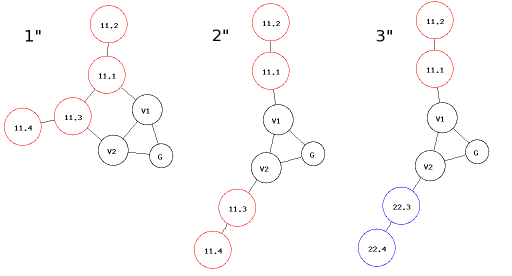
\includegraphics[scale=0.5]{fig/congnode}
	\end{center}
	\caption{In the first step we have the gnode 11.* (in red). In the
	second, the gnode becomes broken. In the third, after the procedure
	described above has been applied, we have two gnodes: 11.* and 22.*}
	\label{fig:congnode}
\end{figure}

\subsection{Compact gnodes}
A gnode $G$ is compact if, fixed a rem value $\ove r$, 
\eal{&\forall a,b\in G\;\;rem(a\stackrel{*}{\rightarrow} b)\le \ove r}
where $a\stackrel{*}{\rightarrow} b$ is the best path from $a$ to $b$.\\
The gnodes don't necessary need to be compact, however the more compact they
are, the more the grouping approximation is reduced (see \ref{groupapprox}).

An optimal technique to keep the gnodes compact hasn't been found yet. As an
example, consider the following, which has been inspired by the gravitational
model: let $n$ be a node and $V_n$ the set of its
neighbours. For each neighbours $v\in V_n$, $n$ calculates the following
\emph{attraction value}:
\eal{&att(v) = \sum_{r\in R_v} rem(r)\\
&\qq\T{ where $R_v$ is the set of all the best routes of $n$ passing from $v$}
}
$n$ is then attracted by the neighbour $\ove v$, which has the highest
attraction value: $n$ will enter in the gnode of $v$ (if it isn't already in).

The problem with any Compact gnodes system is that the grouping of nodes
becomes dependent on the quality of the links, thus the network may be
reconfigured more often.

\section{TODO}
\begin{enumerate}
	\item Answer question \see{questiongn}.
\end{enumerate}
\section{ChangeLog}
\begin{itemize}
	\item \verb|July 2008|
		Changed the term ``fractal'' with ``hierarchical''.
	\item \verb|August 2007|
		\begin{enumerate}
			\item Hooking procedures redesigned, probably they are
				near to their definitive form:
				\begin{enumerate}
					\item The grouping of nodes is now
						handled by the communicating
						vessels system
					\item The case where a gnode is
						split in two parts is managed
						in a less complicated way
					\item a ``gravitational model'' for
						the Compact gnodes has been
						proposed.
				\end{enumerate}
		\end{enumerate}
	\item \verb|July 2007|
		\begin{enumerate}
			\item Internal and external map structure redisigned:
				(see \ref{sec:intmyopia})
			\item The bnode map is no more necessary.
			\item Flat levels simplified.
			\item The hooking procedure has been fused with the
				rehooking preocedure.
			\item Removed section ``Level 0''.
		\end{enumerate}
	\item \verb|March 2007|
		\begin{itemize}
			\item Description of the Flat levels (sec. \ref{sec:flat})
			\item Section ``Network dynamics - Level 0'' expanded.
			\item Section ``Network
				dynamics - Level n'' updated: the references to
				the pre-Flatlevels REM metric have been
				removed.
		\end{itemize}
	\item \verb|October 2006|\\
		Initial release.
\end{itemize}

%%%%%%%%%%%%%%%%
% Bibliography %
%%%%%%%%%%%%%%%%
\begin{thebibliography}{99}
	\bibitem{qspndoc} QSPN document:
		\href{http://netsukuku.freaknet.org/doc/main\_doc/qspn.pdf}{qspn.pdf}
	\bibitem{ntksite} Netsukuku website:
		\href{http://netsukuku.freaknet.org/}{http://netsukuku.freaknet.org/}
	\bibitem{CIDR} CIDR routing:
		\href{http://en.wikipedia.org/wiki/Classless\_Inter-Domain\_Routing}{Classless\_Inter-Domain\_Routing in Wikipedia}
	\bibitem{ntkp2p} P2P over Ntk:
		\href{http://netsukuku.freaknet.org/doc/main\_doc/ntk\_rfc/Ntk\_p2p\_over\_ntk.pdf}{P2P over Ntk}
	\bibitem{caurout} Caustic routing:
		\href{http://lab.dyne.org/Ntk\_caustic\_routing}{RFC 0013}
\end{thebibliography}
\newpage

\begin{center}
\verb|^_^|
\end{center}
\end{document}
